The exponential growth of data-intensive applications is pushing computational hardware to its limits. With silicon transistors nearing their physical limits, scaling is increasingly reliant on \emph{parallel architectures} and \emph{heterogeneous integration}~\cite{iyerHeterogeneousIntegrationPerformance2016}. Efficient data movement is critical in today's hyperscale systems, as large-scale machine learning models require communication over distances where electrical signaling becomes energy-prohibitive. Optical interconnects offer a compelling solution, leveraging distance-agnostic losses and high parallelism~\cite{millerRationaleChallengesOptical2000}. Particularly, Silicon photonics (SiPh) enables scalable optical transceivers using cost-effective, precision tooling developed over decades for the electronics industry~\cite{sorefPresentFutureSilicon2006}. After modest initial growth, SiPh has recently achieved large-scale integration of millions of optical components on a single chip~\cite{shekharRoadmappingNextGeneration2024}, unlocking opportunities at the intersection of photonics, electronics, and computing systems. During my Ph.D. and postdoc, I contributed significantly to SiPh in areas including electronic-photonic design automation (EPDA)~\cite{wuCompactModelingCircuitlevel2017,zhangCompactModelingSilicon2017,jamesFlexibleProcessAwareCompact2022,jamesProcessVariationAwareCompact2023a}, variation characterization and mitigation~\cite{wuPairingMicroringbasedSilicon2018,wangEnergyefficientChannelAlignment2018,wangTamingEmergingDevices2019,wangBidirectionalTuningMicroringbased2019,wangCharacterizationApplicationsSpatial2020,wangEnergyEfficiencyYield2021}, broadband filters and dispersion engineering~\cite{wangDispersionEngineeredFabricationRobustSOI2023,wangIntegratedCompactTunable2023,parsonsOFC25}, ultra-scalable link architectures~\cite{wangScalableArchitectureSubpJ2023,novickHighbandwidthDensitySilicon2023}, automated link control~\cite{wangAutomatedTuningRingAssisted2024,wangInterleaverTuning,wangOFC25}, channel-dependent optimization~\cite{novickIntegratedPhotonicResonant2024,gopalEqualization2024}, network-application co-optimization~\cite{wangTaskMappingAssistedLaser2019,wangTrafficAdaptivePowerReconfiguration2021,michelogiannakisEfficientIntraRackResource2023,wuWavelengthReconfigurableTransceiver2024,wuFlexibleSiliconPhotonic2024}, and photonics-enabled data processing~\cite{naumanOFC25,zypmanDSP}.

\begin{wrapfigure}[44]{r}{0.4\textwidth}
    \vspace{0.1em}
    \begin{center}
        \includegraphics[width=\linewidth]{../../6_figures/rs_fig_1_empho_3dpho.png}
    \end{center}
    \caption{(a)~FOM comparison between pluggable, existing CPO, and my research, showing key enablers of FOM leaps toward future goal. Data sources given in~\cite{wangCoDesignedSiliconPhotonics2024}. (b)~Illustrative integration stack with pluggable optics. (c)~Illustrative integration stack with CPO and our 96\,Tbps MCP prototype. (d)~Envisioned 3D-integrated compute node with embedded photonics directly driven by processor/memory chips. (e)~Conceptual illustration of future multi-chip system enabled by dense 3D optical connectivity.}
    \label{fig:embedded_photonics}
\end{wrapfigure}

Most notably, my postdoctoral research at \mySchoolShort{} was pivotal in demonstrating the first hybrid 2.5D/3D integration of photonic input/output (I/O) chiplets with flip-chip bonded electronic drivers and a field-programmable gate array (FPGA)~\cite{wangSiliconPhotonicsChip2024,wangCoDesignedSiliconPhotonics2024,RovinskiISCAS25}. This prototype achieved unparalleled shoreline bandwidth density and energy efficiency using Kerr comb\textendash{}driven dense wavelength-division multiplexing (DWDM) and advanced packaging. These results advanced the link figure of merit (FOM) by two orders of magnitude over existing co-packaged optics (CPO) solutions (Fig.~\ref{fig:embedded_photonics}a) and led to subsequent funding from government and industry partners. The work has also fostered extensive collaborations with leading industrial partners and academic institutions, enabling the refinement of system prototypes and exploration of transformative connectivity paradigms.

\section*{Transforming Chip-to-Chip Connectivity}

Today's computing clusters face significant connectivity bottlenecks as data bandwidth decreases with distance. Conventional pluggable optical transceivers (Fig.~\ref{fig:embedded_photonics}b) are limited by high power consumption and area overheads for EO/OE conversion. As part of the DARPA PIPES program, I led the photonics design of an optical I/O chiplet architecture leveraging Kerr frequency combs to enable massive wavelength parallelism. This architecture delivered a bidirectional bandwidth exceeding 32\,Tbps with a 4\,Tbps/mm shoreline bandwidth density. Collaborating with Intel and Cornell University, I co-developed a multi-chip package (MCP) integrating photonics, electronics, and a compute chip (Intel Stratix 10 FPGA), achieving a 96\,Tbps bidirectional bandwidth at a sub-pJ/bit energy consumption (Fig.~\ref{fig:embedded_photonics}c)\textemdash{}a two-order-of-magnitude improvement in link FOM, defined as the bandwidth density\textendash{}energy efficiency product. These results have led the successful transition of the DARPA PIPES program into Phase 3, and substantially contributed to the winning of an SRC JUMP 2.0 and a Samsung GRO grant. In these subsequent projects, I have identified a clear pathway to another order of magnitude improvement in the link FOM through on-chip laser integration and wafer-scale substrate undercut, marking a significant leap toward the goal in Fig.~\ref{fig:embedded_photonics}a. As we have demonstrated a truly CMOS-compatible driving voltage (<\,0.4\,V) for the modulators, an exciting future extension to this work comes from a processor/memory chip 3D-integrated with the photonic I/O and directly driving the modulators. This envisioned architecture (Fig.~\ref{fig:embedded_photonics}d) aligns optical channel data rates with processor/memory speeds, allowing for efficient pooling of spatially-distanced resources and eliminating data locality concerns in large-scale parallel computing workloads.

Looking further ahead, I aim to explore a new paradigm of chip-to-chip connectivity that lifts the restrictions of today's planar optical routing, notably the one-dimensional (shoreline) and two-dimensional (areal) chip footprints and fiber array sizing. To enable connectivity scaling, I envision a dense 3D optical system architecture (Fig.~\ref{fig:embedded_photonics}e) that enables any-to-any interconnections from waveguide arrays on an active chip to those on another active chip via an interposer-like routing chip. The photonic chips can be integrated via metal-metal hybrid bonding, enabling high-density electrical connections for power delivery and control signaling, while
additionally providing high alignment accuracy and robust mechanical stability for minimal optical misalignment. The conceptual design of such a system, which I jointly conceived with my collaborators at \mySchoolShort{},
was well received at the 2023 DARPA ERI Summit. This would open up numerous collaboration opportunities across the system stack, including device, packaging, integration, system architecture, and design automation, to realize the next generation of integrated photonic systems with unprecedented density, efficiency, and connectivity.

\section*{Computing within Data Movement}

\begin{wrapfigure}[19]{r}{0.46\textwidth}
    \vspace{-5em}
    \begin{center}
        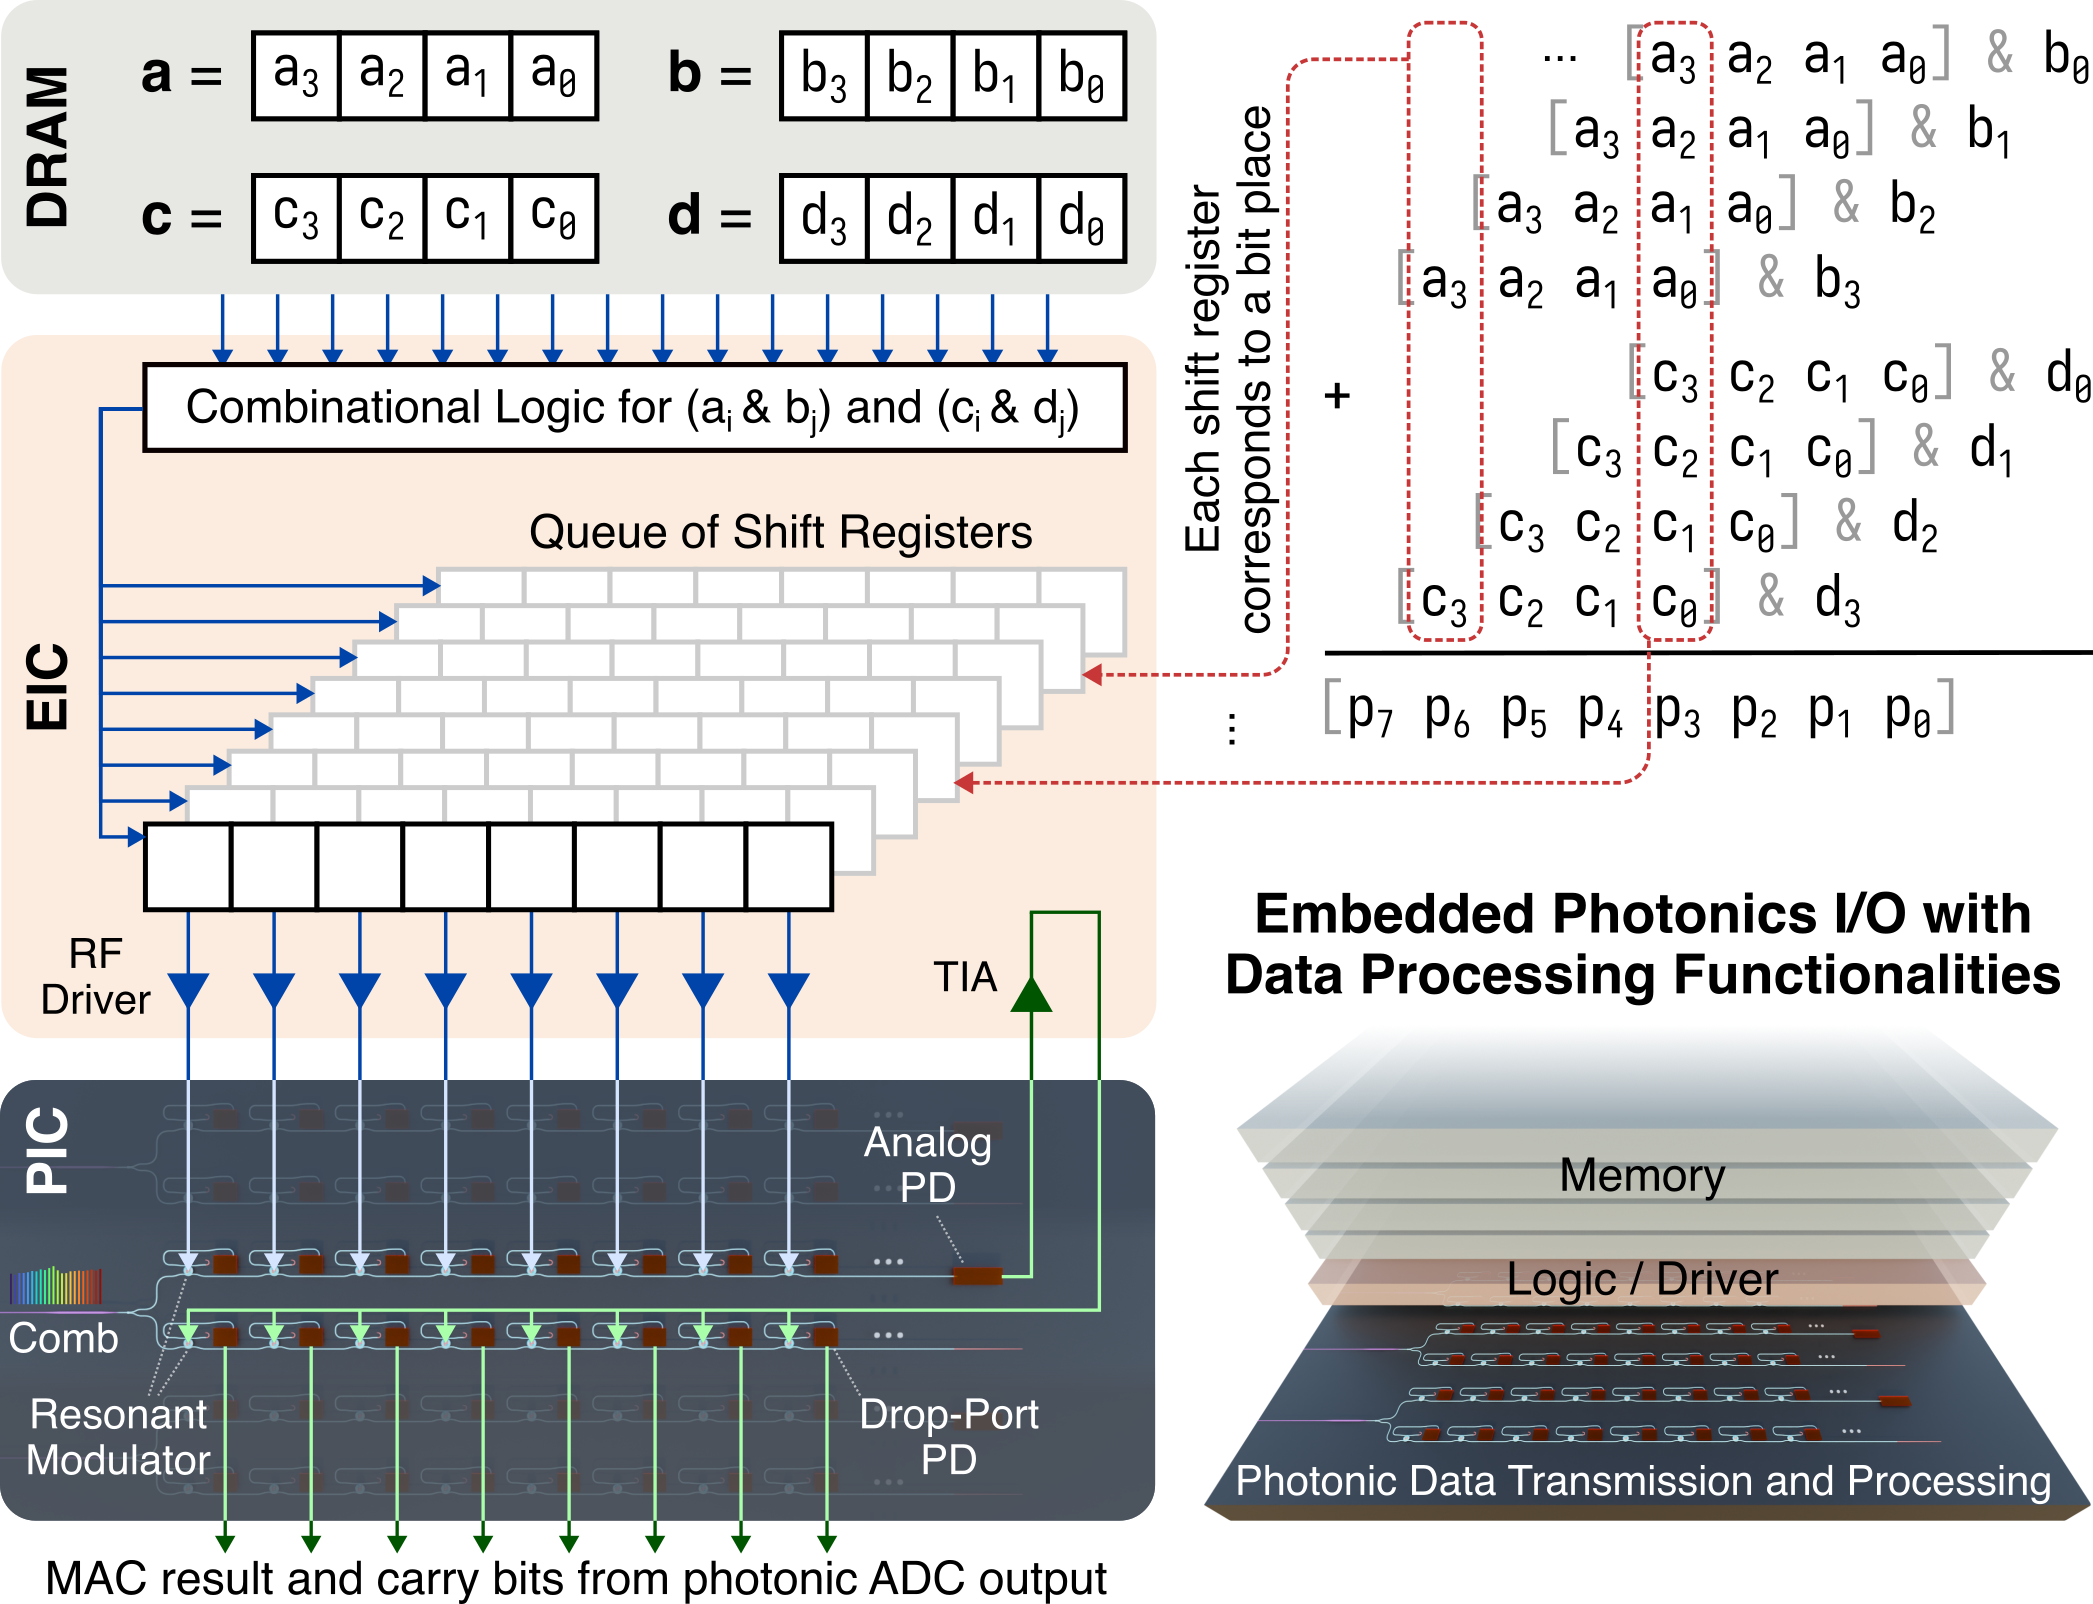
\includegraphics[width=\linewidth]{../../6_figures/rs_fig_3_comppho.png}
    \end{center}
    \caption{Illustration of the photonics-enabled data processing architecture for achieving full-digital-precision MAC operations leveraging comb-driven DWDM and photonic ADC.}
    \label{fig:pho_computing}
\end{wrapfigure}

With SiPh processes reaching reasonable maturity, various novel applications beyond data communication are emerging. A particular category breaks the traditional boundary between communication and computation by leveraging the analog nature of optical signals for operations like vector-vector and matrix-vector multiplications~\cite{taitMicroringWeightBanks2016,shenDeepLearningCoherent2017}. However, current approaches face challenges with scalability, precision, and control complexity, in addition to the need for digital-to-analog and analog-to-digital conversions at the input/output of these architectures.

To address these, a similar architecture to the earlier DWDM transceiver can be repurposed to perform multiply-accumulate (MAC) operations as data is in motion. As shown in Fig.~\ref{fig:pho_computing}, this architecture encodes each bit place of the MAC result as an analog light intensity and counts the number of 1's through a photonic analog-to-digital converter (ADC). Most uniquely, the architecture directly interfaces with the logic die of the memory chip, taking digital representations of the multipliers/multiplicands and the MAC result as input and output, respectively. Bits precision is determined by the number of parallel wavelengths, rather than the granularity of phase shifters. As each wavelength is modulated either on or off, the architecture is inherently more robust to fabrication variations and environmental perturbations. A hardware validation of this architecture is submitted to OFC'25, which demonstrates its efficacy for incorporating data processing into the communication pipeline. Along this line, I am actively exploring the potential of integrating photonic data processing with not only DWDM, but also other architectures such as mode division multiplexing (MDM). Building on my prior experience in advanced packaging and heterogeneous integration, the ultimate goal is to develop a combined photonic I/O\textendash{}processor chip embedded within the package where data is stored/generated. In this architecture, data requesters will fetch computation results directly, rather than raw data. This approach minimizes data movement, reduces latency, and improves energy efficiency by performing computations where data resides and avoiding unnecessary EO/OE conversions between communication and computation. The envisioned architecture initiates a shift in computing paradigm and also finds applications in emerging fields beyond AI/machine learning, such as using photonic data links as the back plane of large-scale antenna arrays and perform signal processing while data is in motion.

\section*{Ecosystem, Funding, and Collaborations}

To achieve the ultimate goal of large-scale integrated photonics involves leveraging the ``fabless'' silicon photonics ecosystem. Over the past few years, I have participated in nine tape-outs with three commercial foundries, including a dedicated 300\,mm run with AIM Photonics where I co-led the design and aggregation. Throughout these experiences, I have developed the necessary knowledge and network to lead a research group that leverages the fabless model. Moreover, my \myDegree{} work in compact modeling partially laid the foundation of EPDA, which equipped me with the skills and mindset to contribute to the development of an ``open'' process design kit (PDK) for the mutual benefit of the SiPh community.

My involvement in DARPA and ARPA-E projects, both of which advanced to Phase 3, has given me valuable experience with program reviews and direct engagement with program managers, providing insights into the critical elements of successful proposals and the criteria for advancement through program phases. I have also been deeply involved in the CUbiC Center under the SRC JUMP 2.0 program, collaborating with PIs from 15 universities and liaisons from 15 industry sponsors, building a strong foundation for future partnerships. Furthermore, I have contributed to over ten research grant proposals in the past two years, including four successful ones from government and industry. Recently, I helped prepare two large-scale CHIPS Act proposals to advance photonic I/O packaging and develop a digital twin for its design and integration process. I believe these extensive experiences will provide me with a competitive edge in acquiring external funding through a deep understanding of the key characteristics of successfully-funded proposals.

My close relationships across academia will provide immediate research avenues that expand on previous work and enable entirely new directions. At \appSchoolDeptShort{}, I additionally envision the opportunity for new collaborations with the current faculty at \appSchoolShort{}, including:
\begin{enumerate*}[label=(\roman*)]
    \appCollab{}
\end{enumerate*}
I am excited to contribute my experience
and enthusiasm to your esteemed institution, keenly anticipating the chance to work with a community that resonates my commitment to making a meaningful impact on the future of computing.